\documentclass[conference]{IEEEtran}
\IEEEoverridecommandlockouts

\usepackage{cite}
\usepackage{amsmath,amssymb,amsfonts}
%\usepackage{algorithmic}
\usepackage{graphicx}
\usepackage{textcomp}
\usepackage{xcolor}
\usepackage{rotating}
\usepackage{bm}
\usepackage{multirow}

\usepackage{algorithm}
\usepackage[noend]{algpseudocode} 

\def\BibTeX{{\rm B\kern-.05em{\sc i\kern-.025em b}\kern-.08em
    T\kern-.1667em\lower.7ex\hbox{E}\kern-.125emX}}
    
% A shortcut for µRTS
\newcommand{\mRTS}{$\mu$RTS}

\begin{document}

\title{Enhancing MCTS Performance in Real-Time Strategy Games Through Move Pruning\\
\thanks{This work has been supported in part by projects B-TIC-402-UGR18 (FEDER and Junta de Andaluc\'{i}a), RTI2018-102002-A-I00 (Ministerio Espa\~{n}ol de Ciencia, Innovaci\'{o}n y Universidades), projects TIN2017-85727-C4-{1-2}-P (Ministerio Espa\~{n}ol de Econom\'{i}a y Competitividad), and TEC2015-68752 (also funded by FEDER).}
}
% Antonio - add here your grants also

\author{\IEEEauthorblockN{Abdessamed Ouessai}
\IEEEauthorblockA{\textit{Dept. Computer Sciences} \\
\textit{University of Mascara}\\
Mascara, Algeria \\
abdessamed.ouessai@univ-mascara.dz\\
ORCID: 0000-0002-1305-8602}
\and
\IEEEauthorblockN{Mohammed Salem}
\IEEEauthorblockA{\textit{Dept. Computer Sciences} \\
\textit{University of Mascara}\\
Mascara, Algeria \\
salem@univ-mascara.dz\\
ORCID: 0000-0001-7052-5978}
\and
\IEEEauthorblockN{Antonio M. Mora}
\IEEEauthorblockA{\textit{Dept. Signal Theory, Telematics and Communications} \\
\textit{ETSIIT-CITIC, University of Granada}\\
Granada, Spain \\
amorag@ugr.es\\
ORCID: 0000-0003-1603-9105}
}


%\title{Enhancing MCTS Performance in Real-Time Strategy Games Through Move Pruning}
%
%\author{
%\IEEEauthorblockN{Abdessamed Ouessai\IEEEauthorrefmark{1}, Mohammed Salem\IEEEauthorrefmark{1} and Antonio M. Mora\IEEEauthorrefmark{2}}
%
%\IEEEauthorblockA{\IEEEauthorrefmark{1}Dept. of Computer Sciences, University of Mascara, Algeria.\\
%abdessamed.ouessai@univ-mascara.dz, salem@univ-mascara.dz}
%
%\IEEEauthorblockA{\IEEEauthorrefmark{2}Dept. of Signal Theory, Telematics and Communications, ETSIIT-CITIC, University of Granada, Spain.\\
%amorag@ugr.es}
%}

\maketitle

\begin{abstract}
The impressive performance of Monte Carlo Tree Search (MCTS) based game-playing agents in high branching-factor domains such as Go, motivated researchers to apply and adapt MCTS to even more challenging domains. Real-time strategy (RTS) games feature a large combinatorial branching factor and a real-time aspect that pose significant challenges to a broad spectrum of AI techniques, including MCTS. Various MCTS enhancements were proposed, such as the combinatorial multi-armed bandit (CMAB) based sampling, state/action abstractions, and machine learning. In this paper, we propose to employ move pruning as a way to improve the performance of MCTS-based agents in the context of RTS games. We describe a class of possibly detrimental player-actions and propose several pruning approaches targeting it. The experimentation results in \mRTS{} indicate that this could be a promising direction.
\end{abstract}

\begin{IEEEkeywords}
Monte Carlo Tree Search, Move Pruning, Real-Time Strategy, Game AI, \mRTS{}
\end{IEEEkeywords}


% -------------------------------------------- INTRODUCTION ------------------------------------------

\section{Introduction}
\label{sec:introduction}

The complexity of real-time strategy (RTS) games, from an AI perspective, originates from the combinatorial structure of their state and decision spaces. In comparison with classic benchmark games such as Chess or Go, the dimensionality of both state and decision spaces in an RTS game is many orders of magnitude higher \cite{ontanon_survey_2013}. Instead of controlling a single unit in a turn-based fashion, RTS players control multiple units simultaneously in real-time, and usually in a much larger board (map) size. Moreover, the branching factor in an RTS game grows exponentially with the increase in the number of units positioned on the map.

Due to the game's complexity, conceiving a human-challenging RTS game-playing agent is a difficult task to undertake. The predominant approach followed by researchers and practitioners in the domain is to decompose the task into manageable subtasks targeting various degrees of abstraction. Most commonly, an RTS agent combines high-level strategic components and low-level tactical components. Such decomposition is inspired by the way human players interweave micro- and macro-management, and it is shown to be effective by numerous implementations \cite{barriga_combining_2017}, \cite{moraes_asymmetric_2018}, \cite{neufeld_hybrid_2019}. 

Holistic search-based approaches such as Monte Carlo Tree Search (MCTS) \cite{browne_survey_2012} enjoyed a remarkable success in computer Go, as demonstrated by AlphaGo \cite{silver_mastering_2016}.
% Antonio - Include some other successful aplications of MCTS to game solving or to game agents' AI. It has been used not only for Go. This is important to remark why we have chosen MCTS as a reference for this study, even if almost all the people in this area will know about its value. ;D
 However, in RTS games, MCTS-based agents struggle with the enormous decision space and fail to scale suitably when the branching factor grows past a certain threshold. Such downside restricts MCTS applicability to limited scenarios, such as tactical planning or small maps. Abstracting the decision space is a tried and tested technique for scaling MCTS-based agents to larger scenarios \cite{ontanon_survey_2013}, 
% Antonio - add a reference to this asseveration, if possible
at the expense of sacrificing tactical performance due to the coarser actions considered.

We propose an approach to increase the performance and scalability of search-based techniques, particularly MCTS-based, by pruning unnecessary and detrimental player-actions from the decision space of an RTS game. 
% Antonio - To be applied by an autonomous agent (as a part of its AI engine)
We inspect the low-level structure of the search space and identify detrimental player-actions through domain knowledge. Next, we apply multiple hard-pruning approaches to remove those player-actions during the search. The goal is to reduce the branching factor and explore more promising player-actions. Our approach targets a class of player-actions we identify as Inactive Player-Actions (IPAs) because they tend to keep at least one unit in an inactive state, which can be problematic. The experiments' results using UCT (Upper Confidence bounds for Trees) and NaïveMCTS in \mRTS{} show a considerable performance gain relative to the map's size.

% Antonio - You should justify why have you chosen IPAs instead of any other possible action 
% Antonio - you haven't mentioned UCT before. I have done it. ;)
 

The rest of this paper is organized as follows: Section \ref{sec:background} reviews some background knowledge about RTS games, \mRTS{} and MCTS. Section \ref{sec:state_of_the_art} presents the related state of the art and Section \ref{sec:proposed_method} describes IPAs and the proposed move pruning approaches. Experimental results are presented and discussed in Section \ref{sec:experiments}, and Section \ref{sec:conclusions} concludes the paper with some conclusions and future perspectives.

% -------------------------------------------- BACKGROUND ------------------------------------------

\section{Background}
\label{sec:background}

\subsection{Real-Time Strategy Games}

A sub-genre of strategy video games, real-time strategy games usually simulate a warfare situation where each side of the game is given control over a military base and is tasked with collecting resources and recruiting troops.
% Antonio - There are RTS with other features, so I would add 'commonly'
 To emerge victorious, the player must fully destroy his opponent's forces. RTS games progress in real-time, signifying that players may act simultaneously under a very short decision cycle, and the effect of executing an action is not necessarily immediate. Usually, an RTS game is played from a top-down perspective over a large grid-based map, covered by a fog-of-war layer reducing observability and increasing the game's difficulty and complexity. Moreover, the execution of a unit-action can be influenced by some stochastic parameters,
% Antonio - could you clarify this? What stochastic parameters do you refer to? ;)
 introducing non-determinism to the mix. Players control their units by issuing unit-actions to each. A player-action is the combination of unit-actions issued simultaneously in the same game cycle.
 
% The combination of unit-actions issued simultaneously at a given game cycle is known as a player-action.

A typical RTS game is defined as a zero-sum, multi-player, non-deterministic game with imperfect information. The size of an RTS state space and branching factor, as estimated in a typical \textsc{StarCraft} setting \cite{ontanon_survey_2013}, reaches $10^{1685}$ possible states and $10^{50}$ possible actions at a decision point. In contrast, Chess and Go possess a state-space estimate of $10^{47}$ and $10^{171}$, respectively, with an average branching factor equaling $36$ in Chess and $180$ in Go. Such proportions predict a difficult task for an RTS game-playing AI.

Based on the terminology and definitions presented in \cite{ontanon_combinatorial_2017}, an RTS game can be defined formally as a tuple $G$, where $G = (S, A, P, \tau, L, W, s_{init})$ and:

\begin{itemize}
\item $S$ : The set of all possible states (state space).
\item $A$ : The set of player-actions (decision space).
\item $P$ : The players set, where $P=\{max,min\}$ for a 2-player setting.
\item $\tau : S \times A \times A \rightarrow S$ : The state transition function. It takes a game state in time $t$ and the player-actions of both players and returns a new game state in $t+1$.
\item $L: S \times A \times P \rightarrow \{true,false\}$ : Determines the legality of a player-action in a given state for a specific player.
\item $W: S \rightarrow P \cup \{ongoing,draw\}$ : Determines the winner of the game or if the game is a draw or is still ongoing.
\item $s_{init} \in S$ : The initial state.
\end{itemize}

% ===========================================

\subsection{\mRTS{}}

Conducting AI research on commercial RTS games can be a daunting experience since most games do not offer a suitable API for this purpose. To mitigate this shortcoming several independent solutions were developed, such as ORTS, the \textsc{WarCraft} port, Wargus, and the unofficial \textsc{StarCraft} interface, BWAPI. Much later, an official API and toolset for \textsc{StarCraft II} were made available in a collaborative effort between Blizzard and DeepMind \cite{vinyals_starcraft_2017-1}. Additionally, several independent RTS AI research platforms have emerged, such as \mRTS{} \cite{ontanon_combinatorial_2017}, ELF \cite{tian_elf:_2017} and DeepRTS \cite{andersen_deep_2018}.

In this paper, we use \mRTS{} as an experimentation test-bed. It is a stripped-down RTS game simulator designed for AI research, which features all the challenging aspects of an RTS game in a minimalistic form. It also includes an efficient forward model, required for implementing simulation-based search approaches. Figure \ref{mRTSScreenshot} shows a screen capture of a \mRTS{} match. Each player controls 2 types of structures (Base and Barracks) and 4 types of mobile units (Worker, Light, Ranged, and Heavy). The Base produces Worker units, and the Barracks produce assault units, in exchange for resources. Worker units can harvest resources from resource deposits and store them in the Base. The game map is an arbitrary-sized 2D grid where each square is either free or occupied by a unit, a structure, or an environment unit (resource deposit or wall).

% Antonio - How is the attack implemented in uRTS? I mean, is it a simple 'unit by unit' elimination when they fight (I guess, when they move to a neighbour cell where it is placed an enemy)?

\begin{figure}[t]
\begin{center}
	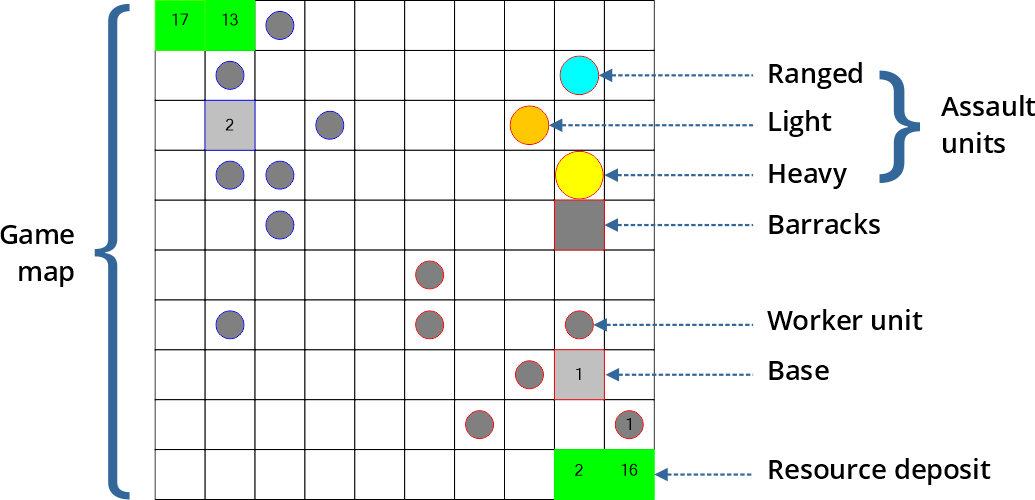
\includegraphics[scale=1]{figs/mRTS.png}
	\caption{A \mRTS{} match. A player's units can be distinguished by their outline's color. The digits displayed over certain units represent the number of resources held by that unit.}
	\label{mRTSScreenshot}
\end{center}
\end{figure}

\mRTS{} represents an interesting research domain for online planning techniques, especially those requiring a forward-model. Several low-level, high-level, and multi-level planning approaches were proposed in \mRTS{} as detailed in \cite{ouessai_online_2019}.

% ===========================================

\subsection{Monte Carlo Tree Search (MCTS)}

The goal of an RTS game-playing agent is to compute an optimal player-action $a \in A$ at each decision cycle $t$ where the agent can act. The successive player-actions computed constitute a plan that should lead the agent to victory. Essentially, this translates to a Markov decision process (MDP) under a tight computation budget and a high decision-space dimensionality. MCTS is a sampling-based search framework applicable to MDPs with large decision spaces unapproachable to systematic search techniques. MCTS relies on the execution of a large number of random simulations to estimate the value of actions sampled through a tree-policy. The MCTS algorithm iteratively constructs a game tree by executing a 4-step process at each iteration. The algorithm can be halted anytime to obtain a decision. An MCTS iteration proceeds as follows:

\begin{enumerate}
\item \textit{Selection:} Select a node with unexplored children following a tree policy.
\item \textit{Expansion:} Expand the selected node by creating and attaching a new child node.
\item \textit{Simulation:} Start a simulation (playout) from the new node following a playout policy.
\item \textit{Backpropagation:} Backpropagate the simulation's results starting from the new node up to the root node, updating all the intermediary nodes' statistics (visit count and value) on the way.
\end{enumerate}

The most visited decision is usually the one returned. Given enough computation budget and a proper exploration/exploitation balance in the tree policy, MCTS is guaranteed to find the minimax solution in the limit. The most popular MCTS implementation, UCT (Upper Confidence bounds for Trees), uses the UCB1 formula as a tree policy, treating the selection phase as a multi-armed bandit (MAB) problem \cite{browne_survey_2012}. Although remarkably successful in Go, UCT does not perform as well in RTS games, due to the rapid growth in the branching factor with the increase in the unit count. NaïveMCTS was designed to better handle the combinatorial search space in RTS games by formulating the selection phase as a combinatorial MAB (CMAB) \cite{ontanon_combinatorial_2017}. NaïveMCTS builds on a naïve sampling approach based on a naïve assumption that considers the reward estimate of a player-action as the sum of the reward estimates of the underlying unit-actions. In our experiments, we used both UCT and NaïveMCTS.

% -------------------------------------------- RELATED WORKS ------------------------------------------

% Antonio - I'd prefer "State of the Art" for this section. ;)
%           Anyway, it doesn't matter if it is named "Related Works", but I think we shouldn't separate it into subsecions

\section{State of the Art}
\label{sec:state_of_the_art}

%\subsection{Search Space Reduction}

Dealing with the enormous RTS decision space in the context of MCTS is an open problem continuously receiving contributions. By treating the selection phase as a CMAB, NaïveMCTS effectively adapts MCTS to combinatorial search spaces. Nevertheless, the decision space remains the same, and the algorithm still suffers from high dimensionality. Downsizing the search space's dimensionality is usually done through action abstraction or machine learning.

Abstracting the search space through expert-authored scripts is an effective way to considerably reduce the branching factor. Instead of searching in the low-level player-actions space, Justesen et al \cite{justesen_script-_2014} adapted UCT to search in the space of player-actions suggested by scripts. NaïveMCTS was similarly adapted by Moraes et al \cite{moraes_action_2018} using asymmetric abstractions \cite{moraes_asymmetric_2018} to search in multiple levels of abstraction. Puppet Search \cite{barriga_puppet_2015} employs UCT to search in the space of choice points inserted into scripts. Guided NaïveMCTS (GNS) \cite{yang_guiding_2019} biases the selection phase towards considering scripted actions first. Other search algorithms were also combined with action abstraction, such as local search in Portfolio Greedy Search (PGS) \cite{churchill_portfolio_2013} and minimax in AHTN \cite{ontanon_adversarial_2015}.

Machine learning can be used to guide node selection by learning a tree policy from expert traces. AlphaGo \cite{silver_mastering_2016} employed a CNN-based policy network, trained from a large database of expert Go replays, and improved via a reinforcement learning phase. Later work on AlphaZero \cite{silver_general_2018} fully discarded expert knowledge. Ontañón informed node selection using a learned Bayesian model in InformedMCTS \cite{ontanon_informed_2016}. Yang and Ontañón \cite{yang_extracting_2019} later demonstrated the effectiveness of the C4.5 classifier for such tasks, due to its speed and accuracy.

%\subsection{Move Pruning}

If we adjust our perspective, all the aforementioned approaches can be regarded as move pruning approaches \cite{yang_integrating_2020}. By focusing on a set of promising expert-based player-actions, these approaches effectively prune the search space of all the remaining player-actions, significantly reducing the branching factor. Such a practice can also become unsafe and prone to exploitation, due to the coarser player-actions considered, resulting in a loss of tactical performance. To address this issue, several approaches combining low- and high-level search have emerged, such as \cite{barriga_combining_2017}, \cite{neufeld_hybrid_2019} and \cite{moraes_action_2018}.

Directly pruning the player-actions responsible for weak playing strength can be an alternative approach towards focusing the search on promising actions, without compromising tactical strength. In the context of Chess \cite{heinz_adaptive_1999} and Shogi \cite{hoki_efficiency_2012}, several forward pruning methods such as Null-move pruning and futility pruning were utilized to reduce the branching factor and enhance $\alpha\beta$ search. In Go, a domain-dependent pruning approach was implemented in UCT \cite{huang_pruning_2010-1}, exploiting territory information. Similar MCTS improvements were applied in Hex \cite{arneson_monte_2010}, Havannah, \cite{dugueperoux_pruning_2016} and DeadEnd \cite{he_game_2008-1}. In video-games, Sephton et al \cite{sephton_heuristic_2014} also enhanced MCTS by applying a knowledge-based move pruning approach for the strategic card game, Lords of War.

In this paper, we propose a domain knowledge-based hard-pruning approach for MCTS agents in RTS games, targeting a specific type of player-actions.


% --------------------------------------- PROPOSED MOVE PRUNING METHOD ------------------------------------------

\section{Move Pruning}
\label{sec:proposed_method}

We propose to act directly on the decision space and hard-prune a subset of decisions we deem irrelevant and/or detrimental to the performance of MCTS. By doing so, MCTS will be freed from sampling those decisions and simulating their outcomes. The recovered computation time will be spent on exploring more relevant and significant decisions. Consequentially, the playing strength and scalability of MCTS should be improved.

As a first attempt, we chose to focus on player-actions having the highest chance of misleading search and negatively impacting the playing strength. Out of these player-actions, we believe Inactive Player-Actions (IPAs) naturally come first. Thus, we implemented several pruning approaches that keep a predefined number (fixed or relative) of those player-actions and prune the remaining. We will briefly discuss the structure of RTS player-actions in the next section and then define IPAs.

% ===========================================

\subsection{Unit-Actions and Player-Actions}

In a typical RTS game, each unit type can execute a distinct set of actions known as unit-actions. Table \ref{unitActionsTable} enumerates the unit-action types executable by each unit-type in \mRTS{}. The Worker unit-type is the most versatile, followed by assault units (Light, Ranged and Heavy) and structures (Base and Barracks). The attributes of a unit-type define the effect of its unit-actions. For instance, the damage attribute controls how much damage a unit-type causes when executing the Attack unit-action. Thus, even for common unit-actions, each unit-type may behave differently. All unit-action types, except Wait, require an argument that determines the target of the action. The Wait unit-action type requires a numeric argument specifying the number of cycles ahead at which the unit must remain inactive. Wait is the only unit-action type unaffected by unit attributes and executable by all unit-types.

\begin{table}[!t]
\renewcommand{\arraystretch}{1.3}
\caption{The unit-action types available for each unit-type in \mRTS{}}
\label{unitActionsTable}
\centering
\begin{tabular}{c|c|c|c|c|c|c}
\cline{2-7}
\multicolumn{1}{c|}{} & Move & Attack & Harvest & Return & Produce & Wait \\
\hline \hline
Worker   & $\bullet$ & $\bullet$ & $\bullet$ & $\bullet$ & $\bullet$ & $\bullet$ \\
%\hline
Light    & $\bullet$ & $\bullet$ & & & & $\bullet$ \\
%\hline
Ranged   & $\bullet$ & $\bullet$ & & & & $\bullet$ \\
%\hline
Heavy    & $\bullet$ & $\bullet$ & & & & $\bullet$ \\
%\hline
Base     & & & & & $\bullet$ & $\bullet$ \\
%\hline
Barracks & & & & & $\bullet$ & $\bullet$ \\
\hline
\end{tabular}
\end{table}

A player-action $p \in A$ issued to $n$ units at a given game cycle can be regarded as a tuple, where $p = (a_1, a_2, \dots, a_n)$ and each component $a_i$ represents a unit-action issued to the same-indexed unit. Assuming each unit is assigned a valid and legal unit-action, and given the average number of unit-actions available to each unit, $m$. The number of all possible player-actions or the branching factor, $b$, can be estimated as $b = m^n$. We seek to lower $b$ by finding ways to decrease $m$ without negatively impacting the playing strength.

% ===========================================

\subsection{Inactive Player-Actions}

We define an Inactive Player-Action (IPA) as a player-action having at least one Wait (inactive, idle, no-op) unit-action as a component. Being the most prevalent non-critical unit-action, Wait unit-actions make for a good pruning target. The Wait unit-action is continuously available to all units, regardless of their situation. Thus, it strongly contributes to the inflation of the search space. Nonetheless, Wait unit-actions can be advantageous for a unit, usually in the following situations:

\begin{itemize}
\item \textit{Trapped unit:} No active unit-action is possible. The unit is caught in a situation where all possible unit-actions are illegal. Waiting for a predefined duration is the only option to choose in hopes the situation is resolved.
\item \textit{Tactical waiting:} The unit anticipates for a chance to execute a high-value unit-action. Here, the unit expects a sub-optimal action by an opponent unit (via lookahead) and chooses to Wait in anticipation for it. Executing the high-value action happens afterward. This behavior is frequently observed in tactical skirmishes.
\end{itemize}

Although potentially useful, Wait unit-actions can also have a devastating effect on the playing strength if improperly chosen. According to our observations, it is not unlikely for a search-based agent (MCTS or otherwise) to assign a Wait unit-action to a unit in a situation where better options exist. In such cases, doing nothing is the worst decision possible. We identify three disadvantageous situations where Waiting cannot be a sound decision:

\begin{itemize}
\item \textit{Waiting in front of opportunity:} Here, the unit can seize an immediate opportunity, such as Harvest resources, Return harvested resources, or safely remove an opponent unit. Instead, the unit is assigned Wait.
\item \textit{Waiting in face of danger:} The unit is facing an immediate danger and holds the necessary options to avoid it, but instead, it is assigned a Wait unit-action.
\item \textit{Waiting frequently:} The unit is assigned Wait unit-actions more often than the other unit-actions, in the absence of immediate dangers/opportunities, making it less effective in pursuing opportunities and almost passive.
\end{itemize}

The presence of one Wait unit-action in a player-action (thus, IPA) is enough to introduce a risk of encountering one of the disadvantageous situations. The more Wait unit-actions in an IPA, the higher this risk gets. Thus, we believe that pruning all IPAs from the search space, while preserving some IPAs as a safety measure to account for trapped units and tactical waiting, can be beneficial to MCTS.

%Out of place, Wait unit-action assignments, can exhibit a similar effect to noise, and sampling-based search approaches can be distracted away from more interesting options.

% ===========================================

\subsection{Pruning Techniques}

The radical pruning approach would be to remove all IPAs from the search space, basically removing the Wait unit-action from the set of unit-actions of all unit types. Thus, diminishing $m$ by $1$ and obtaining a branching factor $b' = (m - 1)^n$, which represents a considerable decline from $b$. As an example, if we have $m=5$ unit-actions on average in a given game state with $n=6$ units, then $b \approx 1.56\times10^4$ and $b' \approx 4\times10^3$. The total number of IPAs removed would be: $v = b - b' = 1.16\times10^4$. The reduction is significant, but we intend to keep a portion of IPAs to deal with trapped units and tactical waiting.

% Pruning Analysis results, moved in this section to appear in the same 
% page as the relevant section.
\begin{figure*}[!h]
\begin{center}
	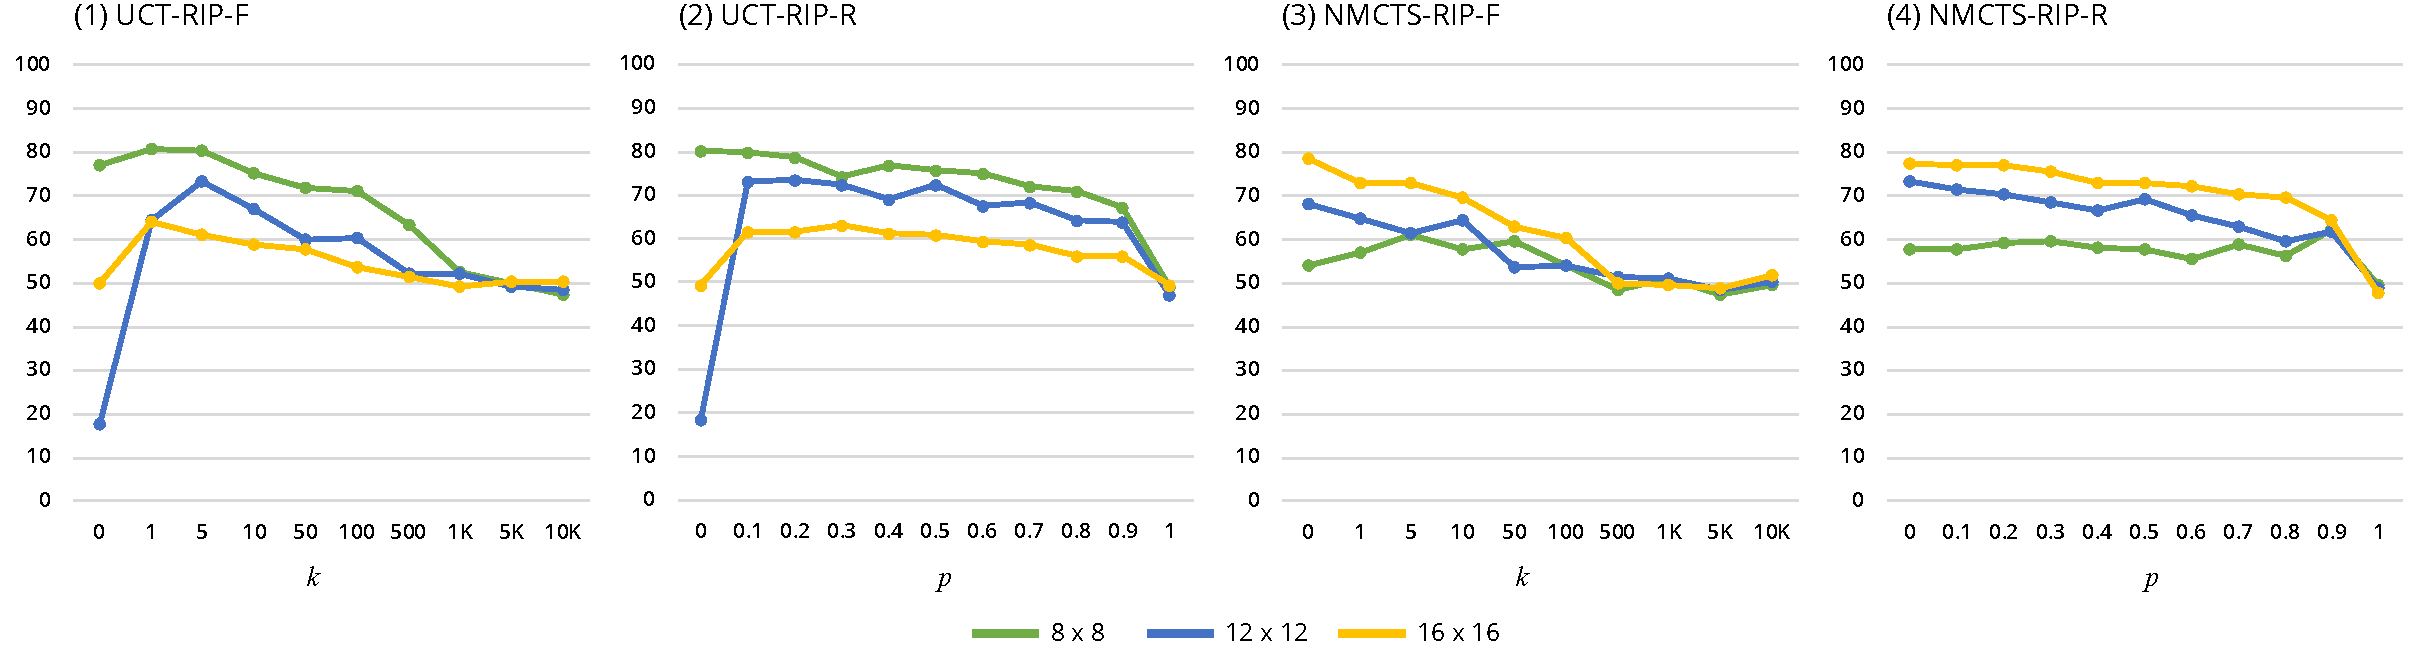
\includegraphics[width=1\textwidth]{figs/PT-h.pdf}
	\caption{Results of the pruning analysis experiments. Each data point represents $500$ matches between the basic MCTS agent and the one augmented with IPA pruning. The vertical axes represent the score obtained by the IPA pruning MCTS agent against the same non-pruning MCTS agent. The score is calculated as such: $score = ((Wins + (Draws / 2)) / 500) \times 100$. A match is considered a draw if no winner has been decided after $3000$, $3500$, and $4000$ cycles in each map of size $8\times8$, $12\times12$, and $16\times16$, respectively.}
	\label{PruningAnalysis}
\end{center}
\end{figure*}

Detecting trapped units is a simple task. But dealing with tactical waiting can be elusive since there is no simple way to differentiate between waiting as a tactical choice, and waiting as a bad decision until witnessing the consequences. Random playouts do not offer a reliable answer in that regard. We propose four pruning approaches that capture IPAs and decide whether to allow or prune them according to a given parameter. These approaches preserve all IPAs involving trapped units and allow a predetermined number/rate of random IPAs in hopes of preserving tactical waiting situations. The remaining IPAs are all considered disadvantageous and are systematically hard-pruned. We do not re-insert pruned IPAs because we consider the non-pruned player-actions more urgent to explore. The pruning approaches are described as follows:

\begin{itemize}
\item \textbf{Random Inactivity Pruning - Fixed (RIP-F($k$)):} Allow a fixed number $k$ of IPAs.
\item \textbf{Random Inactivity Pruning - Relative (RIP-R($p$)):} Allow a percentage of IPAs $p$ relative to the total number of removable IPAs.
\item \textbf{Dynamic RIP-F (DRIP-F($k_1$, $k_2$)):} Allow $k_1$ IPAs when the units count outnumber the opponent's units count, and $k_2$ IPAs in the opposite situation.
\item \textbf{Dynamic RIP-R (DRIP-R($p_1$, $p_2$)):} Allow $p_1$ percent of IPAs when the units count outnumber the opponent's units count, and $p_2$ percent of IPAs in the opposite situation.
\end{itemize}

The intuition behind dynamic approaches is to equalize the chances of performing tactical waiting when the agent does not hold a numerical advantage. This is done by allowing more IPAs when the agent is outnumbered ($k_2 > k_1$ or $p_2 > p_1$).

These approaches can be easily implemented as part of any search algorithm, as shown in Algorithm 1. \textsc{isIPA($a$)} returns true if at least one Wait unit-action exists in $a$, and \textsc{TrappedUnit($a$)} returns true if $a$ includes a Wait unit-action involving a trapped unit. \textsc{CheckParam()} returns true if a parameter-check decides to disallow (prune) the player-action. The approaches differ in \textsc{CheckParam()} implementation.

%They operate by capturing player-actions while sampling and checking whether an IPA was captured or not. In case the IPA does not involve a trapped unit, a parameter check decides whether to prune the IPA or allow it. If pruned, the search algorithm must sample another action while keeping track of the pruned IPAs. 

%In the next section, we report the experiments conducted and the results obtained by enhancing UCT and NaïveMCTS with these pruning approaches in the context of RTS games.

\begin{center}
\scalebox{0.9}{ 
\begin{minipage}{1\linewidth}
\begin{algorithm}[H]
\label{pruningAlgorithm}
\caption{The general IPA pruning algorithm.}
\begin{algorithmic}[1]
\Function{Prune}{$a$} \Comment{$a:$ sampled player-action}
	\If{ \textsc{isIPA($a$)}}
		\If{\textsc{TrappedUnit($a$)}} \textbf{return} $a$ \EndIf
		\If{$a\in$ \textit{prunedIPAs} \textbf{or} \textsc{CheckParam()}}
			\While{\textsc{isIPA($a$)}}
				\State \textit{prunedIPAs.addIfNotExist}($a$)
				\State $a\gets$ \textsc{SampleAction}(gameState)
			\EndWhile
		\EndIf
	\EndIf
	\State \textbf{return} $a$
\EndFunction
\end{algorithmic}
\end{algorithm}
\end{minipage}}
\end{center}


% --------------------------------------- EXPERIMENTATION AND RESULTS ------------------------------------------


\section{Experimentation and Results}
\label{sec:experiments}

%\begin{figure*}[!h]
%\begin{center}
%	\includegraphics[width=1\textwidth]{figs/WLR.pdf}
%	\caption{Win / Loss / Draw Ratios}
%	\label{WLR}
%\end{center}
%\end{figure*}

To study the effect of pruning IPAs on MCTS, we implemented the four aforementioned pruning techniques in UCT and NaïveMCTS and conducted various experiments in \mRTS{}. Indeed, UCT's performance suffers greatly in RTS scenarios due to UCB1's limitations in combinatorial search spaces \cite{ontanon_combinatorial_2017}, nevertheless we wanted to test if pruning IPAs would alleviate the dimensionality burden and results in performance improvement. Integrating IPA pruning into UCT and NaïveMCTS generated new agents that we refer to by suffixing the acronym of the technique to that of the original search approach. For instance, the agent using RIP-R with UCT or NaïveMCTS is noted as UCT-RIP-R($p$) or NMCTS-RIP-R($p$).

We first analyzed the performance of RIP-F and RIP-R relative to the number of IPAs allowed, the map's size, and the MCTS algorithm in use. We then took the top-performing pruning approaches for each MCTS algorithm and map size and performed a round-robin tournament with other \mRTS{} agents. Afterward, we examined the impact on the branching factor and performed a scalability test in larger maps. The experiments were carried out on two PCs with Intel Core i5 and i7 CPUs, clocked at 3.1Ghz and 3.4Ghz, respectively, using the latest version of \mRTS{} at the time of writing.

% ===========================================

\subsection{Pruning Analysis}

To analyze the influence of IPA pruning on the performance of MCTS, we ran a series of experiments involving each MCTS agent and non-dynamic IPA pruning approach. We defined two distinct sets, $F$ and $R$, composed of a selection of values that can be taken by the parameters of RIP-F($k$) and RIP-R($p$), respectively. Next, we ran $500$ matches (switching sides after $250$ matches) between the MCTS agent enhanced with an IPA pruning approach, and the non-pruning version of the same MCTS agent for each respective value in $F$ or $R$. The process was repeated for each \textit{basesWorkers} map of size $8\times8$, $12\times12$ and $16\times16$. We define $F$ and $R$ as follows:

\begin{itemize}
\item $F = \{0, 1, 5, 10, 50, 100, 500, 1000, 5000, 10000\}$
\item $R = \{0, 0.1, 0.2, 0.3, 0.4, 0.5, 0.6, 0.7, 0.8, 0.9, 1\}$
\end{itemize}

The total number of matches played for a single MCTS agent amounts to $(500\times\vert F\vert\times3) + (500\times\vert R\vert\times3)$, yielding $63000$ matches for both UCT and NaïveMCTS. In all experiments, we kept the default UCT and NaïveMCTS parameters as defined in \mRTS{} codebase, for all variants. Agents were given $100ms$ per frame as a computation budget. The experiment results are expressed in Figure \ref{PruningAnalysis}'s plots.

Overall, we can see that IPA pruning is responsible for a performance gain of variable rates, relative to the number of IPAs allowed and the branching factor represented by the map's size. In UCT-RIP-F, allowing a small number of IPAs ($0 < k \leq 5$) significantly increases UCT's performance. However, the more IPAs are allowed, the more performance decreases until pruning losses its effect ($k \geq 1000$). The same trend is witnessed in UCT-RIP-R. Allowing a small percent of IPAs ($0.1 \leq p \leq 0.3$) increases UCT's performance, but the more we raise $p$ the more performance drops. We note that UCT-RIP-R($p=1$) and UCT-RIP-F($k \geq 1000$) are equivalent to non-pruning UCT.

The highest performance gain was recorded in the smallest $8\times8$ map with the lowest branching factor, and the lowest gain was recorded in the largest $16\times16$ map. This is expected from UCT since its sampling strategy (UCB1) is highly prone to combinatorial search spaces. Thus, pruning IPAs is not enough to scale UCT's performance. Pruning all IPAs ($k = 0$ or $p = 0$) hurts UCT's performance in larger maps due to the large number of IPAs encountered. This causes frequent player-action re-samplings that rapidly consume the computation budget, leaving very little time to exploitation. Although this effect is offset in the $16\times16$ map by the large number of draws, it is quite clear in the $12\times12$ map.

From the perspective of NaïveMCTS, IPA pruning exhibits the same effect as in UCT, with two key differences. First, in the smallest $8\times8$ map, NaïveMCTS performs optimally when more IPAs are allowed, that is, when $5 \leq k \leq 50$ in NMCTS-RIP-F and $p=0.9$ in NMCTS-RIP-R. This is probably because naïve sampling already handles small scenarios well and can gain an advantage if a portion of IPAs is kept to explore tactical waiting situations. However in larger maps, pruning all IPAs ($k = 0$, or $p = 0$) yields the highest performance gain. Here, due to the bigger branching factor, pruning IPAs significantly contributes to the better utilization of the computation budget.

The second difference with respect to UCT is the scalability of performance, relative to the increase in the branching factor. As opposed to UCT, NaïveMCTS enhanced with IPA pruning delivers its best performance in the largest $16\times16$ map, followed by the $12\times12$ map. Having fewer IPAs in the search space seems to allow naïve sampling to sample more interesting player-actions, instead of wasting time on IPAs. Moreover, pruning IPAs increases the movement frequency of units, resulting in an enhanced ability to explore large maps and to discover interesting opportunities. We will see further how this translates to larger maps.

% ===========================================

\subsection{Best Pruning Approaches}

Concerning dynamic pruning approaches (DRIP-F and DRIP-R), we have conducted a similar experiment using UCT, by fixing $k_1$ (or $p_1$) to the optimal $k$ (or $p$) value found for each map size and performing $500$ matches for each $k_2$ (or $p_2$) value from $F$ (or $R$). We omitted the results because of space constraints. For NaïveMCTS, dynamic pruning did not bring any improvement over non-dynamic approaches, based on preliminary tests. Thus, performing extensive experiments was not necessary. The best performing IPA pruning approaches for each map-size and MCTS algorithm are shown in Table \ref{bestApproaches}.

\begin{table}[!h]
\renewcommand{\arraystretch}{1.3}
\caption{Best Performing Pruning Approaches}
\label{bestApproaches}
\centering
\resizebox{1\columnwidth}{!}{
\begin{tabular}{c|c|c||c|c||c|c}
\cline{2-7}
\multicolumn{1}{c|}{} & $8\times8$ & Score & $12\times12$ & Score & $16\times16$ & Score  \\ 
\hline \hline
UCT & DRIP-F(1,0) & $82.2$ & DRIP-R(0.2,0.4) & $76.8$ & RIP-F(1) & $63.9$ \\
NaïveMCTS & RIP-R(0.9) & $62.3$ & RIP-R(0) & $73.3$ & RIP-F(0) & $78.6$ \\
\hline
\end{tabular}
}
\end{table}

For UCT, dynamic approaches work best in the small and medium-sized maps due to the frequent encounters between opposing units. In the largest map, exploration becomes more urgent, rendering the dynamic approaches ineffective.
% Antonio -  In 16x16 for UCT shouldn't it be DRIP instead of RIP?
%                  Don't you comment these results?

% ===========================================

\subsection{Performance Analysis}

To further assess the performance impact of IPA pruning on MCTS agents, we have run a round-robin tournament between 8 \mRTS{} agents, including two IPA pruning MCTS agents. The tournament consists of 100 iterations, where in each iteration, every agent plays a match against the other agents resulting in $8\times7\times100 = 5600$ matches in each of the maps used previously. The participating \mRTS{} agents include four baseline agents and one top performing agent from 2019's \mRTS{} competition, MixedBot: % Antonio - I guess MixedBot is the top performing agent.:D

\begin{itemize}
\item \textit{NaïveMCTS:} The original unmodified NaïveMCTS.
\item \textit{RandomBiased:} Selects actions randomly, with a bias towards attacking and harvesting.
\item \textit{POWorkerRush:} Continuously produces workers and sends them to attack the opponent.
\item \textit{POLightRush:} Same as the above, but using Light units.
\item \textit{MixedBot:} Relies on two separate agents; Tiamat\cite{marino_evolving_2018} for strategic decisions and Capivara\cite{moraes_action_2018} for tactical decisions. Both based on search space abstraction through scripts and tuned for different map sizes.
\end{itemize}

In addition to the following IPA pruning agents:

\begin{itemize}
\item \textit{NMCTS-RIP:} NaïveMCTS integrating one of the IPA pruning approaches for each relevant map size, as defined in Table \ref{bestApproaches}.
\item \textit{UCT-RIP:} Same as the above, but based on UCT.
\end{itemize}

We also included unmodified UCT for the sake of comparison. The global tournament results are reported in Table \ref{tournamentResults}, and the results by map-size are shown in Figure \ref{TournamentResultsAllMaps}. The score is calculated similarly to the previous experiment, by summing the win count and the half of the draw count.

\begin{table}[!t]
\renewcommand{\arraystretch}{1.3}
\caption{Global Tournament Results (Row agent vs. column agent)}
\label{tournamentResults}
\centering
\resizebox{1\columnwidth}{!}{
\begin{tabular}{r|cccccccc|c}
 & \begin{sideways}NMCTS-RIP\end{sideways} & \begin{sideways}UCT-RIP\end{sideways} & \begin{sideways}NaïveMCTS\end{sideways} & \begin{sideways}UCT\end{sideways} & \begin{sideways}RandomBiased\end{sideways} & \begin{sideways}POWorkerRush\end{sideways} & \begin{sideways}POLightRush\end{sideways} & \begin{sideways}MixedBot\end{sideways} & \begin{sideways}Average\end{sideways}  \\ 
\hline \hline
NMCTS-RIP    & - & $\bm{80.6}$ & $\bm{72.1}$ & $\bm{96}$ & $\bm{100}$ & $42.1$ & $47.3$ & $26$ & $\bm{66.3}$ \\
UCT-RIP      & $20.8$ & - & $30.6$ & {$\bm{78}$} & $\bm{98.1}$ & $26.8$ & $35.5$ & $14.1$ & $43.4$  \\
NaïveMCTS    & $31$ & $\bm{69.3}$ & - & $\bm{94}$ & $\bm{100}$ & $34.5$ & $36.3$ & $9.3$ & $\bm{53.5}$ \\
UCT          & $2.3$ & $21.3$ & $7.5$ & - & $\bm{84.8}$ & $13$ & $34.6$ & $1$ & $23.5$ \\
RandomBiased & $0$ & $1$ & $0$ & $13$ & - & $0$ & $6.6$ & $0$ & $2.9$ \\
POWorkerRush & $\bm{60.6}$ & $\bm{72.3}$ & $\bm{69.8}$ & $\bm{89.5}$ & $\bm{100}$ & - & $\bm{100}$ & $\bm{74.5}$ & $\bm{80.9}$  \\
POLightRush  & $\bm{57.8}$ & $\bm{65.3}$ & $\bm{66.3}$ & $\bm{66.6}$ & $\bm{98.3}$ & $0$ & - & $30.8$ & $\bm{55}$  \\
MixedBot     & $\bm{74.8}$ & $\bm{86.8}$ & $\bm{89.6}$ & $\bm{99}$ & $\bm{100}$ & $30.5$ & $\bm{82}$ & - & $\bm{80.4}$ \\
\hline
\end{tabular}}
\end{table}

\begin{figure}[!t]
\begin{center}
	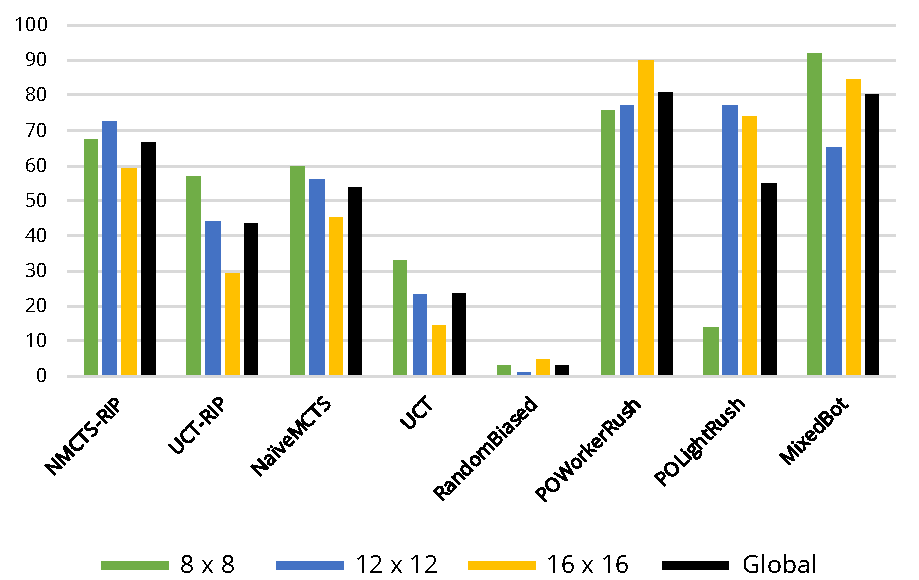
\includegraphics[width=1\columnwidth]{figs/TR.pdf}
	\caption{The tournament results in each of the three map sizes. The vertical axis represents the obtained score against all agents.}
	\label{TournamentResultsAllMaps}
\end{center}
\end{figure}

% Branching factor analysis results - floating table. ---------------------------
\begin{table*}[!t]
\caption{Branching Factor, Sampled Actions and IPA Pruning Statistics}
\label{BranchingFactorTable}
\renewcommand{\arraystretch}{1.3}
\centering
\resizebox{1\textwidth}{!}{
\begin{tabular}{c|c||c|c|c|c||c|c|c} 
\hline
Agent & Map & \begin{tabular}[c]{@{}c@{}}Avg. Branching \\Factor, $b$ (Incl IPAs)\end{tabular} & \begin{tabular}[c]{@{}c@{}}Avg. Unit\\Count, $n$\end{tabular} & \begin{tabular}[c]{@{}c@{}}Avg. Unit-Actions,\\ $m$ (Incl Wait)\end{tabular} & \begin{tabular}[c]{@{}c@{}}Avg. Branching\\Factor, $b'$ (w/o IPAs)\end{tabular} & \begin{tabular}[c]{@{}c@{}}Avg.\\Sampled Actions\end{tabular} & \begin{tabular}[c]{@{}c@{}}IPAs \% in\\Sampled Actions\end{tabular} & \begin{tabular}[c]{@{}c@{}}Pruned IPAs \%\\(WRT Sampled Actions)\end{tabular} \\ 
\hline \hline
\multirow{3}{*}{NMCTS-RIP} & 
   $8\times8$ & $1782$ & $5.19$ & $3.15$ & $54$ & $70.81$ & $33.82\%$  & $6.04\%$  \\
 & $12\times12$ & $2.48\times10^7$ & $14.39$ & $2.67$ & $1561$ & $75.27$ & $71.81\%$ & $14.32\%$            \\
 & $16\times16$ & $9.519\times10^{11}$ & $20.92$ & $3.11$ & $6.12\times10^6$ & $71.25$ & $76.72\%$ & $24.56\%$ \\ 
\hline
\multirow{3}{*}{NaïveMCTS} & 
   $8\times8$ & $784$ & $5.32$ & $2.71$ & $17$ & $71.76$ & $80.03\%$ & $0\%$ \\
 & $12\times12$ & $6.51\times10^6$ & $14.39$ & $2.54$ & $494$ & $80.11$ & $99.24\%$ & $0\%$ \\
 & $16\times16$ & $1.842\times10^{11}$ & $20.06$ & $3.05$ & $1.87\times10^6$ & $76.85$ & $99.88\%$ &  $0\%$ \\
\hline
\end{tabular}}
\end{table*}


The results demonstrate how IPA pruning positively affects the playing strength of UCT and NaïveMCTS. Looking at the average scores, NMCTS-RIP achieved a $12.8$ points increase with respect to NaïveMCTS, and UCT-RIP achieved a near $20$ points increase, relative to UCT. IPA pruning in UCT (UCT-RIP) managed to shrink the performance gap between UCT and NaïveMCTS from $30$ points to $10.1$ points, noticeable in Figure \ref{TournamentResultsAllMaps} where UCT-RIP's performance closely matches that of NaïveMCTS in the $8\times8$ map. Moreover, NMCTS-RIP was able to score a higher average than POLightRush, one of the strongest scripts usually outranking NaïveMCTS. Against each agent, both NMCTS-RIP and UCT-RIP obtained significantly higher scores than those of NaïveMCTS and UCT respectively.

As expected, scripts and script-based approaches exhibit a superior performance versus low-level MCTS search approaches, due to the presence of expert knowledge in the form of hard-coded scripts. Expert knowledge helps in avoiding detrimental player-actions by focusing the search on a limited set of player-actions judged more rewarding. However, this comes at the cost of lower decision granularity and higher exploitation risk. By pruning detrimental player-actions, we hope to focus the search on a wider range of interesting player-actions and keep a higher degree of decision granularity. The fact that NMCTS-RIP could achieve a higher average score than MixedBot in the $12\times12$ map signifies that our approach could be promising.

% ===========================================

\subsection{Branching Factor \& Scalability}

To better grasp how IPA pruning affects MCTS performance, we took $100$ mid-game states from matches between NMCTS-RIP and NaïveMCTS and ran a $100ms$ search, starting from those states for both agents. The search was limited to one ply ($maxDepth=1$), and the mid-game was defined at $400$, $600$ and $1000$ game cycles for each map of size $8\times8$, $12\times12$ and $16\times16$, respectively. The statistics collected during these searches are reported in Table \ref{BranchingFactorTable}.

We can see that the branching factor $b$ in mid-game states is higher in NMCTS-RIP, as a result of the similarly higher unit-actions average $m$. This, in turn, is the consequence of the units being spread out on the map due to lesser IPAs (more movements), leading to more space between units, and more possible actions for each. NMCTS-RIP samples player-actions from a subset of the decision space having a lower bound branching factor $b'$, expanded by the number of IPAs involving trapped units, and a random set of IPAs allowed by the pruning approach.

The rate of IPAs in both branching factor and sampled actions grows proportionally to the branching factor, as expected. The rate of IPAs in sampled actions is significantly high in NaïveMCTS, reaching near $100\%$ in larger maps. Whereas in NMCTS-RIP, this rate drops under $34\%$ and would not go beyond $77\%$ in the tested maps. Moreover, the rate of pruned IPAs increases proportionally with the branching factor. Therefore we may conclude that in larger maps NaïveMCTS gets fully overwhelmed by IPAs, while NMCTS-RIP prunes more IPAs and focuses on a larger number of possibly better player-actions. This further highlights the detrimental effect of the overabundance of IPAs.

We have run $100$ matches (switching sides after 50 matches) between NMCTS-RIP-F($0$) and NaïveMCTS in larger $24\times24$ and $32\times32$ maps, to test the performance scalability of IPA pruning in larger scenarios. The results in Table \ref{largeMaps} suggest a stable score trend and an increasing win/loss ratio proportional to the map's size. Further experiments in these scenarios are planned in the context of our next works.

\begin{table}[!t]
\caption{NMCTS-RIP-F($0$) Results in Larger Maps}
\label{largeMaps}
\renewcommand{\arraystretch}{1.3}
\centering
\begin{tabular}{c|c|c|c|c} 
\cline{2-5}
\multicolumn{1}{c|}{} & Wins & Losses & Draws & Score  \\ 
\hline \hline
$24\times24$ & $52$ & $6$ & $42$ & $73$ \\
$32\times32$ & $43$ & $1$ & $56$ & $71$ \\
\hline
\end{tabular}
\end{table}

% --------------------------------------- CONCLUSIONS AND FUTURE WORK ------------------------------------------

\section{Conclusions and Future Work}
\label{sec:conclusions}

Throughout this paper, we have studied the possibility of employing move pruning as a way to enhance MCTS performance in the context of RTS games. We have identified a class of player-actions that can negatively impact the performance of low-level MCTS approaches. We labeled those actions as Inactive Player-Actions (IPAs) due to their tendency to keep at least one unit in an inactive state. Several pruning approaches were conceived to directly prune IPAs, taking into account the existence of possibly useful IPAs. We then carried out a range of experiments to test the validity of our approaches and discussed the obtained results. According to the results, pruning IPAs is associated with a meaningful performance gain, due to the reduced branching factor and the increased focus on more interesting player-actions. IPA pruning in NaïveMCTS has demonstrated an impressive performance across increasingly larger maps, especially when all excessive IPAs get pruned. Therefore, we conclude that NaïveMCTS can safely ignore all superfluous IPAs in such situations, which will grant a risk-free performance boost.

Move pruning in this context can be seen as "inverse" action abstraction, since we are trying to find the set of player-actions to avoid, whereas, action abstraction methods seek to find the set of player-actions to focus on exclusively. Pruning low-quality player-actions could result in a more flexible and granular decision space, rather than the coarser space induced by action abstractions (scripts).

There are, probably, other types of low-quality player-actions that deserve pruning, such as those involving aimless unit movements. Researching more prunable player-action types falls into the scope of our next work, along with further analysis of IPA pruning in larger scenarios, and the investigation of the impact of IPA pruning in multi-level search approaches such as STT\cite{barriga_combining_2017} and A3N\cite{moraes_action_2018}. Finally, we believe that more research into the low-level structure of the RTS decision space could lead to a deeper understanding of the general features of higher-quality decisions.

%\section*{Acknowledgments}

\bibliographystyle{IEEEtranS}
\bibliography{library}

\end{document}
